L'applicativo, oltre a seguire un design MVC per la separazione e l'organizzazione dei componenti, implementa anche un pattern di comunicazione ad eventi, meglio conosciuto come \textit{pattern observer-delegate}. 

In sostanza, ogni componente che necessita di una certa tipologia di informazioni si mette in ascolto registrandosi ad un "servizio" offerto, nel nostro caso, dal \textit{DataDispatcherSingleton} il quale va a salvarsi al suo interno un gruppo di riferimenti (delegati) che dovrà poi notificare nel momento in cui risulteranno essere presenti nuove informazioni a cui gli observers risultano essere interessati.

Come si può ben capire si tratta quindi di un pattern molto vicino alla struttura \textit{Publish-Subscriber}, con il quale si definisce una dipendenza uno a molti fra gli oggetti: in sostanza abbiamo un oggetto che viene \textit{"osservato"} e tanti oggetti che \textit{"osservano"} i cambiamenti di quest'ultimo, come si può vedere nella struttura generica rappresentata in figura ~\ref{fig:ObserverStructure}.

\begin{figure}[h]
	\centering
	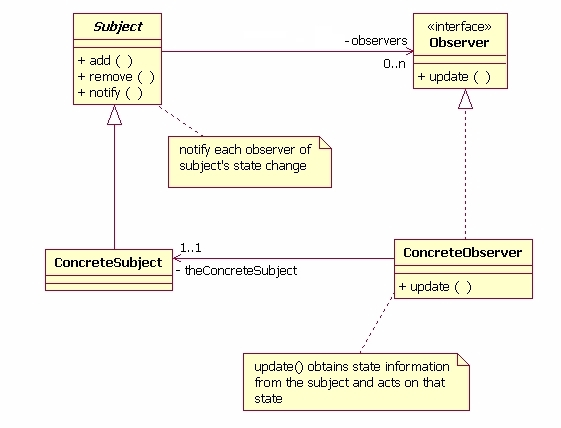
\includegraphics[width=0.5\textwidth]{Immagini/Observer/ObserverTheory.jpg}
	\caption{Struttura generica pattern observer}
	\label{fig:ObserverStructure}
\end{figure}

Questa struttura è stata riprodotta anche nel nostro applicativo, dove è possibile notare la presenza di alcune strutture caratteristiche di questo pattern: abbiamo infatti una funzionalità di \textit{register}, che, a seconda di quale observer richiama questa funzione, pone l'oggetto nel vettore specifico (figura ~\ref{fig:RegisterFunction}). 
Per evitare di avere dipendenze cicliche o comunque per mantenere una certa pulizia nei riferimenti tra classi, è necessario che ogni observer, nel momento in cui non necessita più di una certa tipologia di informazionw, vada a deregistrarsi: questa operazione consiste nell'andare a togliere qualsiasi riferimento dell'oggetto in esame dall'interno del \textit{DataDispatcherSingleton}, come fatto in figura ~\ref{fig:UnregisterFunction}.

\begin{figure}[h]
	\centering
	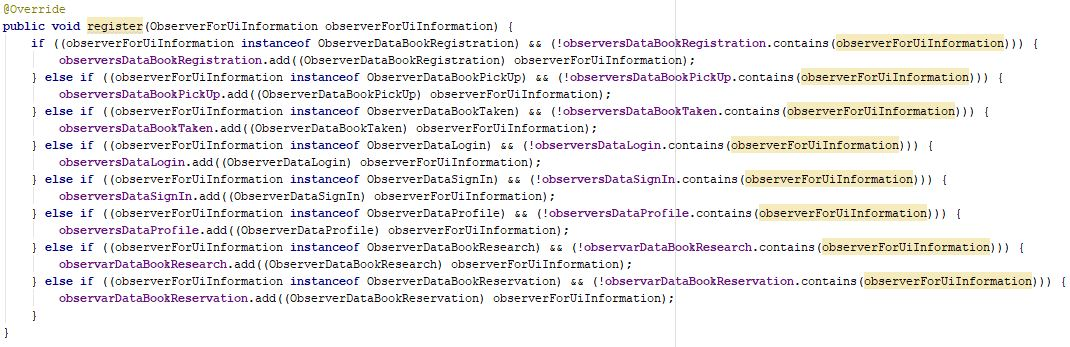
\includegraphics[width=\textwidth]{Immagini/Observer/RegisterToDispatcherData.JPG}
	\caption{Register function}
	\label{fig:RegisterFunction}
\end{figure}

\begin{figure}[h]
	\centering
	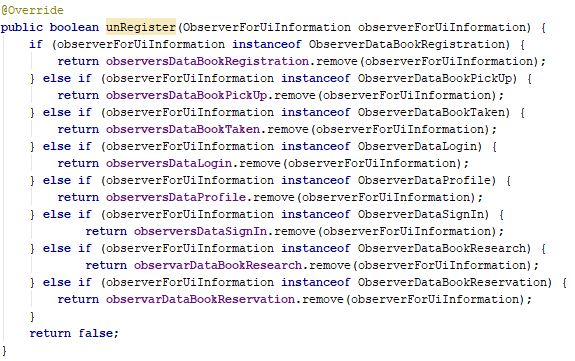
\includegraphics[width=0.8\textwidth]{Immagini/Observer/UnregisterFromDispatcherData.JPG}
	\caption{Unregister function}
	\label{fig:UnregisterFunction}
\end{figure}

Per quanto riguarda invece la parte di \textit{notifica} abbiamo introdotto un pattern ad eventi custom,mantenendo così separata l'implementazione delle informazioni ottenuto da ogni singolo fragment, come si vede nella figura ~\ref{fig:ObserverForUiInformation}.

\begin{figure}[h]
	\centering
	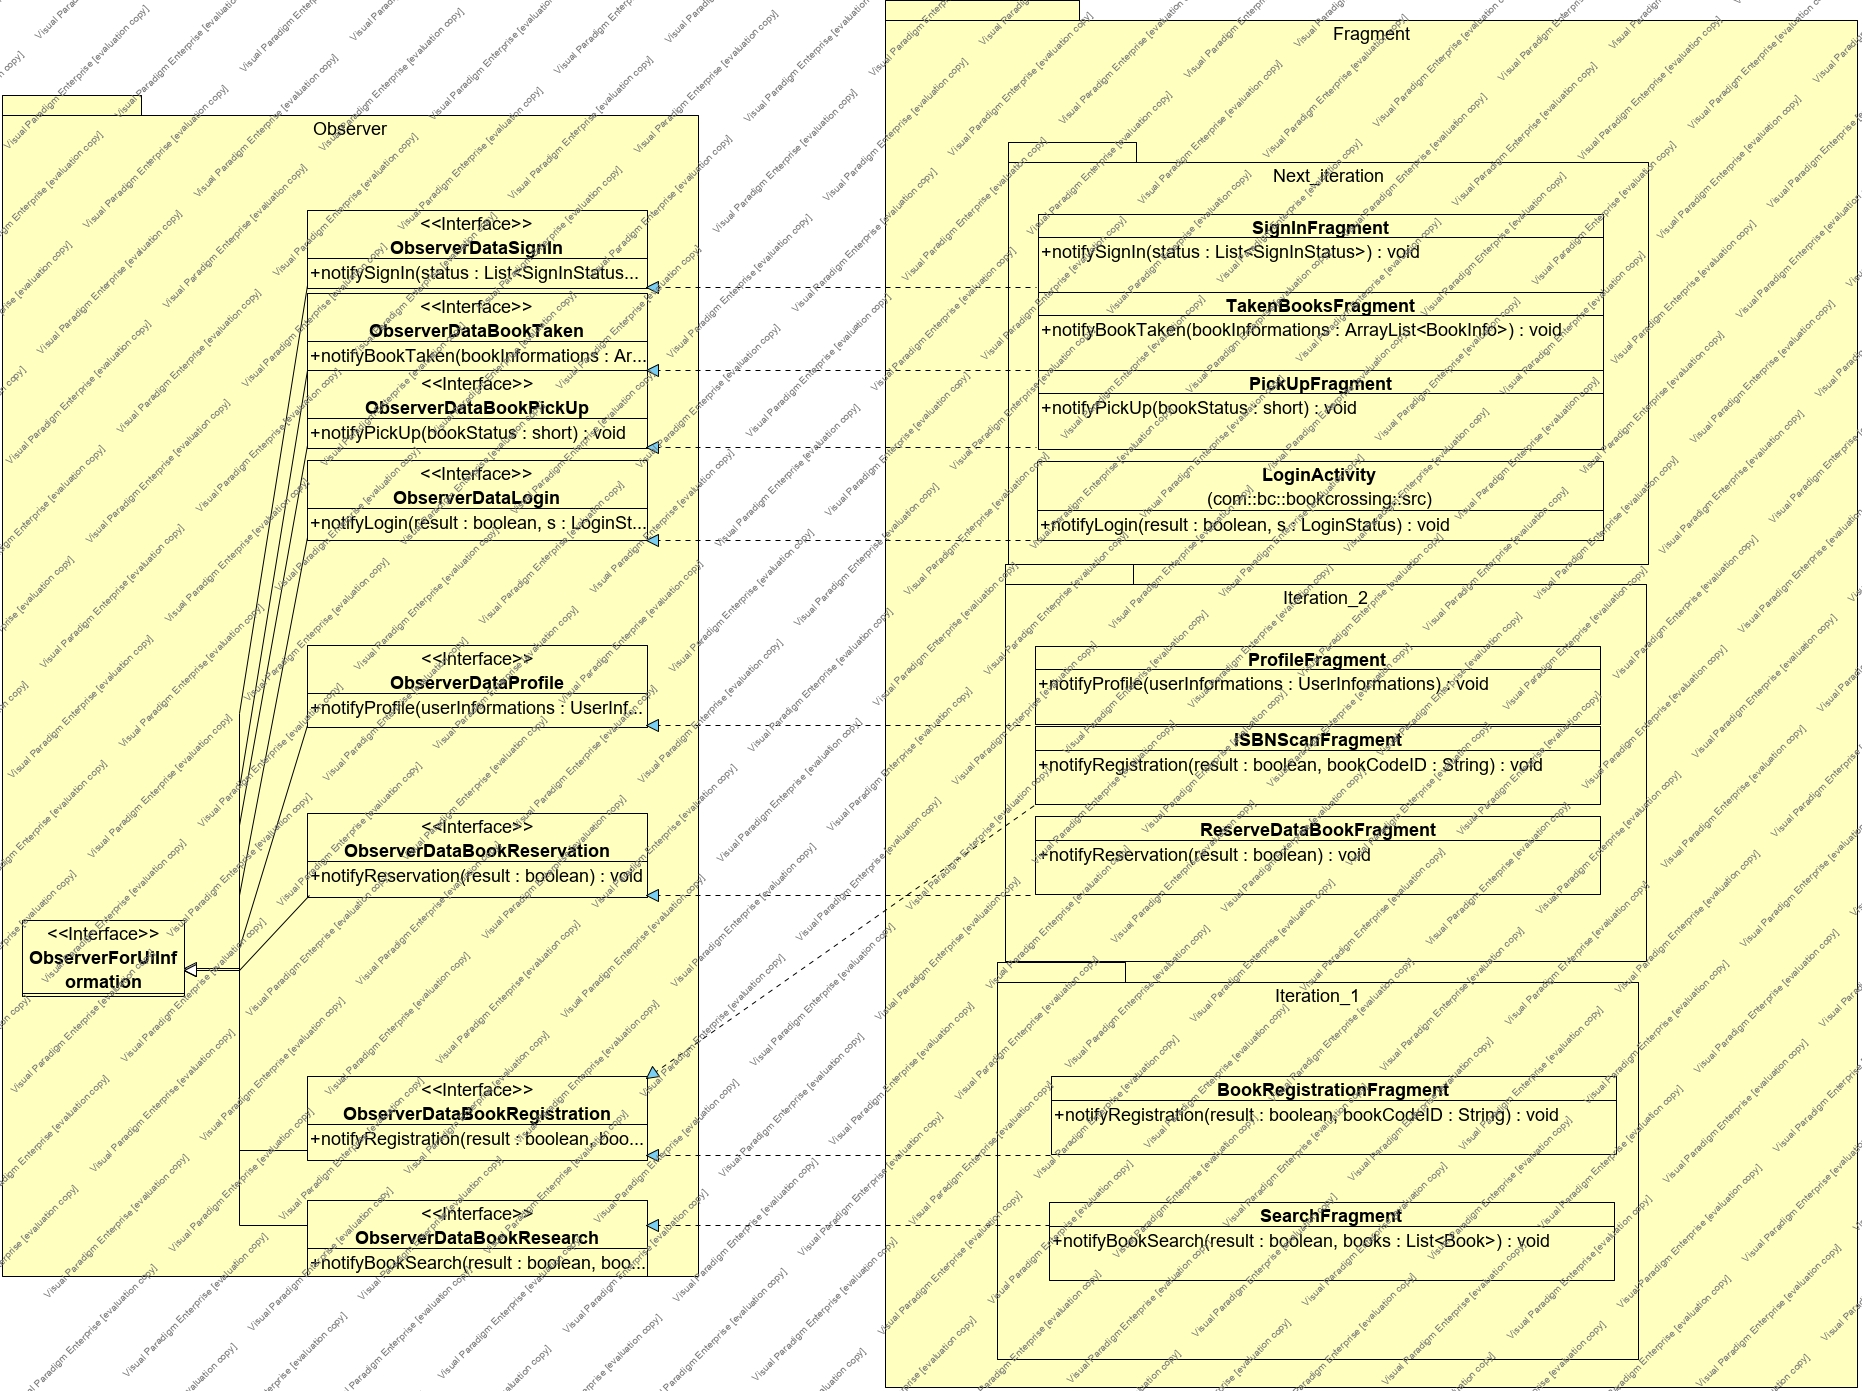
\includegraphics[width=\textwidth]{Immagini/ObserverForUIInformation}
	\caption{Interfaccie per la ricezione degli eventi da lato server}
	\label{fig:ObserverForUiInformation}
\end{figure}

Ogni singola interfaccia implementa a sua volta un'interfaccia comune a più alto livello: questa scelta è stata adotta per rendere del tutto generico il tipo di observer che va a registrarsi per gli eventi forniti dal delegate.

Infatti, come si può vedere nell'interfaccia \textit{DelegateSendData} (figura ~\ref{fig:DataDispatcher}), chi è interessato ad ottenere informazioni specifiche si registra come un oggeto di tipo \textit{ObserverForUiInformation}; sarà poi compito del delegate fornire le corrette informazioni andando a richiamare le corrette funzioni di notifica (direttamente implementate all'interno di ogni singola interfaccia concreta).

\begin{figure}[h!]
	\centering
	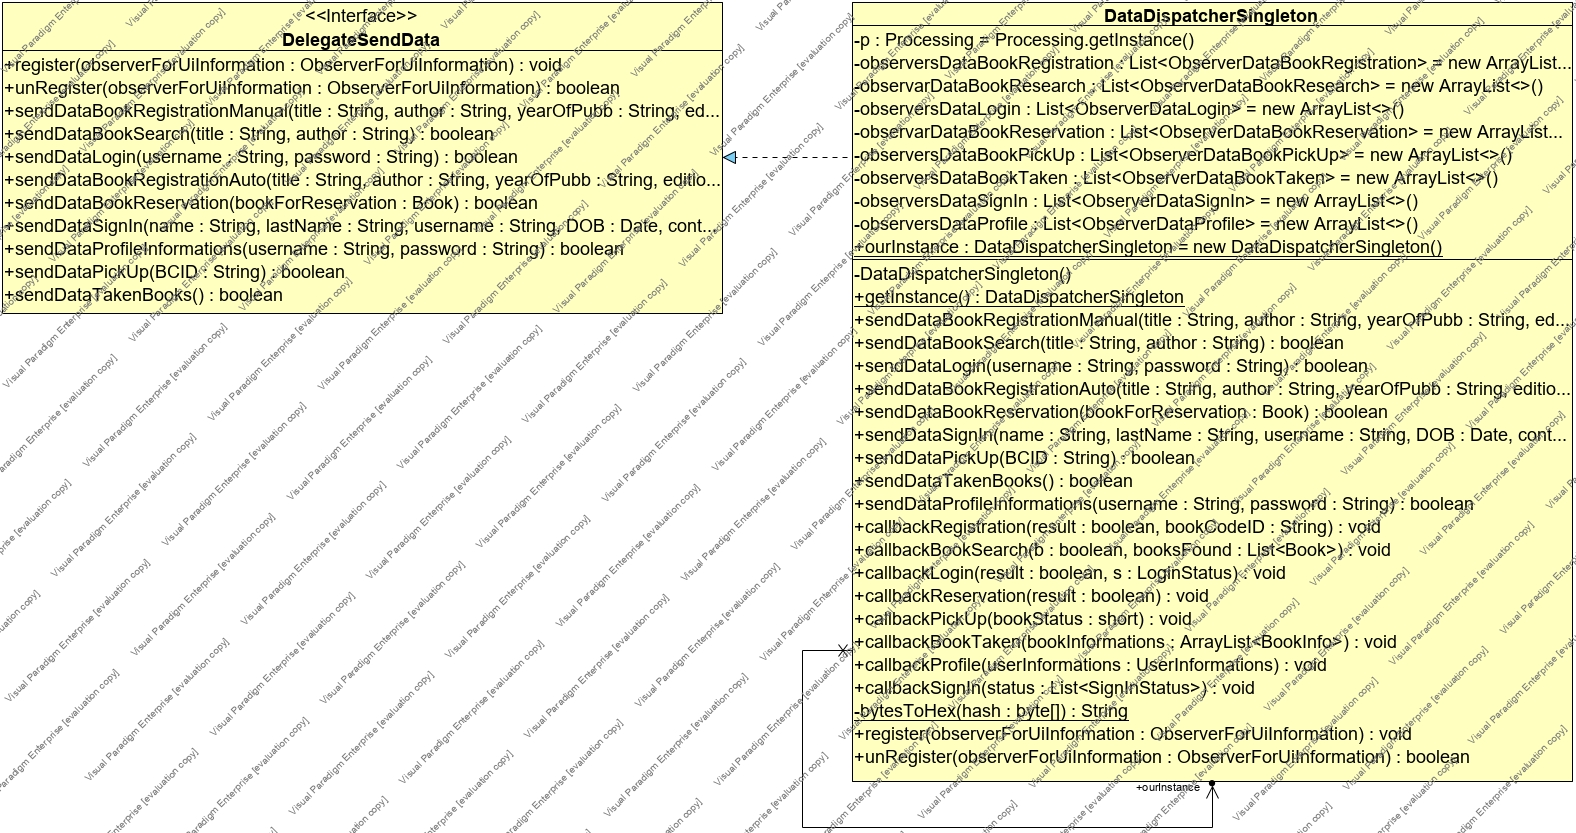
\includegraphics[width=\textwidth]{Immagini/ClassDiagramDispatcherDelegate}
	\caption{Struttura del componente \textit{DataDispatcher}}
	\label{fig:DataDispatcher}
\end{figure}

Si può quindi vedere che, nella struttura predisposta, il \textit{DataDispatcher} lavora come se fosse un \textbf{repository}, ovvero un contenitore di informazioni, in grado di fornire a tutti gli elementi che si registrano i dati di cui necessitano.

Questi elementi, allo stadio implementativo attuale, sono rappresentati da tutti i fragment, che devo ricevere/inviare informazioni per soddisfare l'interazione con l'utente: come si può notare nelle figure ~\ref{fig:LoginFragment}-~\ref{fig:BookRegistrationFragment}-~\ref{fig:BookRegistrationFragment}-~\ref{fig:ReservationFragment}, ogni singolo fragment è predisposto per ricevere le informazioni di cui ha bisogno, tramite la chiamata delle callbacks da parte del dispatcher stesso.


\begin{figure}[h!]
	\centering
	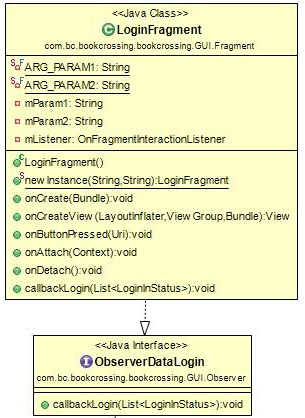
\includegraphics[width=0.5\textwidth]{Immagini/LoginFragment}
	\caption{Struttura del componente \textit{LoginFragment}}
	\label{fig:LoginFragment}
\end{figure}


\begin{figure}[h!]
	\centering
	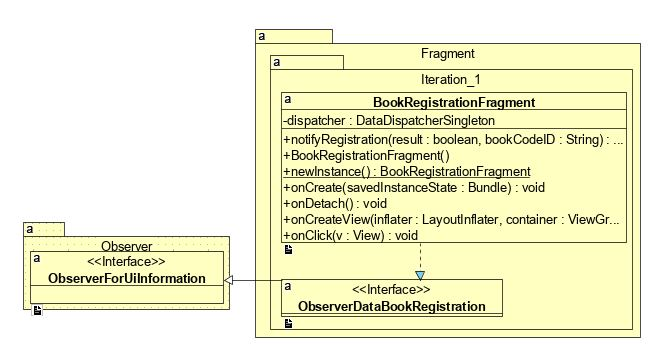
\includegraphics[width=0.5\textwidth]{Immagini/BookRegistrationFragment}
	\caption{Struttura del componente \textit{BookRegistrationFragment}}
	\label{fig:BookRegistrationFragment}
\end{figure}

\begin{figure} [h!]
	\centering
	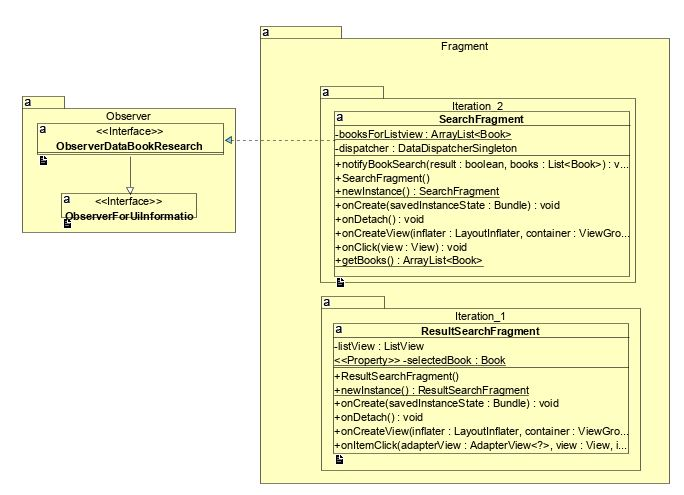
\includegraphics[width=0.5\textwidth]{Immagini/ResearchFragment.jpg}
	\caption{Struttura del componente \textit{ResearchFragment}}
	\label{fig:ResearchFragment}
\end{figure}

\begin{figure} [h!]
	\centering
	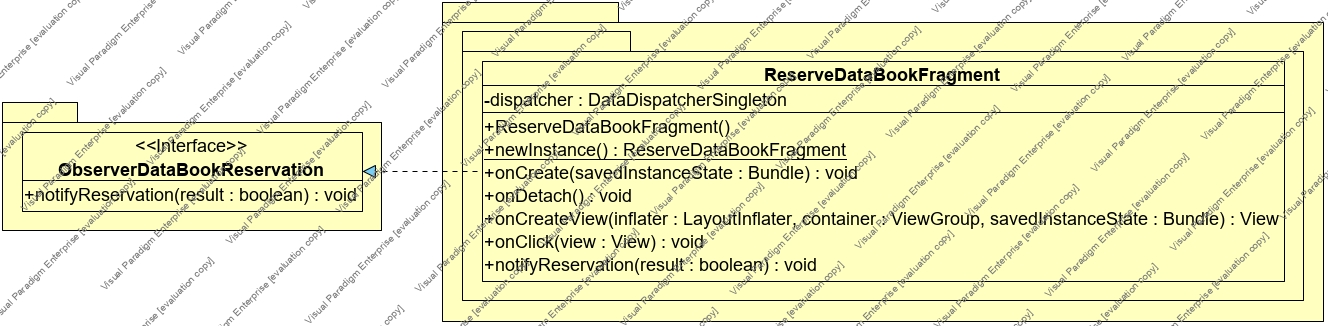
\includegraphics[width=0.5\textwidth]{Immagini/ReservationFragment.jpg}
	\caption{Struttura del componente \textit{ReservationFragment}}
	\label{fig:ReservationFragment}
\end{figure}